\chapter{Background}
\label{ch:background}

Western spatial music emerged during the renaissance period. The
earliest published example of spatial music was by Adrian Willaert in
1550.\cite{Zvonar1999c} The Basilica San Marco, in Venice, where
Willaert was \textit{maestro di capella} had an interesting feature:
Two separate pipe organs facing each other across the
chapel. Willaert took advantage of the organs by composing music for
separate choirs and instrumental groups adjacent the two
organs. Spatial music soon became a fashion, and gradually spread
beyond Venice, as more and more spatially separated groups were
incorporated into composition. However, interest in spatial composition
declined toward the end of the Baroque period, and was largely avoided
until the Romantic period. Beriloz' \textit{Requiem} in 1837, Giuseppe
Verdi's \textit{Requiem} in 1874, and Mahler's \textit{Symphony No. 2}
in 1895 all feature spatially separated brass ensembles.

\section{20th Century Modernism}
\label{sec:modernism}
As the romantic period was coming to an end, there was a blossoming of
complexity, diversity, and invention in contemporary music. Performers
developed the virtuosic skills required to play the music, composers
also wrote increasingly difficult scores to challenge the
performers.\cite{grout2006} Works by Italian composer Luciano Berio
illustrate the complexity of contemporary music of the time. Beginning
in 1958, Berio wrote a series of works he called
\textit{Sequenza}. Each was a highly of highly technical composition
written for a virtuosic soloist. Each was for a different instrument
ranging from flute to guitar to accordion.  In Sequenza~IV, for piano,
Berio juxtaposes thirty-second note quintuplets, sextuplets, and
septuplets (each with a different dynamic), over just a few measures.

\section{Polytempic Music}
\label{sec:background-polytempi}
During the modernist period, composers sought for new ways to
use time and space as compositional elements. Unlike spatial music,
however, polytempic music was comparatively less developed, and many
different polytempic strategies can be found in 20th century
music:
\begin{enumerate}
\item Groups of tuplets layered against a global tempo, as used by
  Henry Cowell (\textit{Quartet Romantic}, 1915-17), and Brian Fernyhough
  (\textit{Epicycle for Twenty Solo Strings}, 1968).
\item Polymeters are notated against a global tempo, and the value of
  a quarter note is the same in both sections, as in Elliott Carter's \textit{Double
    Concerto for Harpsichord and Piano with Two Chamber Orchestras}, 1961
  and George Crumb's \textit{Black Angels}, 1971.
\item Sections are notated without meter. Notes are positioned
  horizontally on the leger linearly according to their position in
  time. Conlon Nancarrow (\textit{Study No. 8 for Player Piano},
  1962), and Luciano Berio (\textit{Tempi Conceriati}, 1958-59).
\item The orchestra is divided into groups, and groups are given
  musical passages with varying tempi. The conductor cues groups to
  begin. Pierre Boulez, \textit{Rituel: In Memoriam Maderna} (1974).
\item One master conductor, directs the entrances of auxiliary
  conductors, who each have their own tempo, and direct orchestral
  sections. This approach was used by Brant Henry in \textit{Antiphony
    One for Symphony Orchestra Divided into 5 Separated Groups} (1953).
\end{enumerate}

\subsection{Charles Ives and The Unanswered Question}
\label{sec:Charles Ives}
Charles Ives' 1908 composition \textit{The Unanswered Question}
incorporates both spatial and polytempic elements. In this piece, the
string section is positioned away from the stage, while the trumpet
solist and woodwind ensemble are on the stage. A dialogue between the
trumpet, flutes, and strings, is written into the music, with the
trumpet repeatedly posing a melodic question \textit{"The Perennial
  Question of Existence''}. Each question is answered by flute
section. The first response is synchronized with the trumpet part, but
subsequent responses accelerate, and intentionally desynchronize with
the soloist. Ives included a note at the beginning of the score which
describes the behavior of the ``answers'':
\begin{quotation}
This part need not be played in the exact time position indicated. It
is played in somewhat of an impromptu way; if there is no conductor,
one of the flute players may direct their playing.

The flutes will end their part approximately near the position
indicated in the string score; but in any case, "The Last Question"
should not be played by the trumpet until "The Silences" of the
strings in the distance have been heard for a measure or two. The
strings will continue their last chord for two measures or so after
the trumpet stops. If the strings shall have reached their last chord
before the trumpet plays "The Last Question", they will hold it
through and continue after, as suggested above.

"The Answers" may be played somewhat sooner after each "Question" than
indicated in the score, but "The Question" should be played no sooner
for that reason.
\end{quotation}
Ives gave the performers license over the temporal alignment, but he
made it clear the parts should not be played together. Following Ives,
other modernist composers also sought new ways to manipulate tempo and
meter. 

\subsection{Gruppen}
\label{sec:gruppen}
Another polytempic example is Karlheinz Stockhausen's \textit{Gruppen}
for three orchestras (1955-57). Parallel tempi that come in and out of
syncronicity is always a challenge with polytempic music, and
Stockhausen found and effective solution. He developed a system of
discrete tempo changes that approximated the logarithmic steps of a
musical scale. Each of the three orchestras was to have it's own
conductor. The conductor would listen for a cue carefully written in
to one of the other sections. That cue would signal to the conductor
to begin beating a silent measure at the new tempo and prepare the new
orchestra to begin playing.

\subsection{New Polytempi}
\label{sec:new-polytempi}
The many different approaches to polytempi in modernist music, all
have one thing in common: They all wrestle with syncronicity. Human
performers, are not naturally equipped to play simultaneous tempi, and
composers must find workarounds to make polytempic performance
accessible. The examples described here exist in one or more of the
following categories:
\begin{enumerate}
\item The music may suggest, multiple tempi, but the beginning and end
  of the individual voices' measures align with each other.
\item The tempo changes are discrete, happening at either measure
  or beat divisions.
\item The tempo changes are somewhat flexible, and  the exact number of
  beats that elapse during a transition varies from one performance to
  another. 

\item The tempo acceleration are linear, and align only at simple
  mathematical relationships.
\end{enumerate}
It is non-trivial to rigorously define parallel tempo curves that
accelerate and decelerate continuously relative to each other, and
come into syncronicity at strict predetermined musical points for all
voices. In \autoref{ch:polytempic}, we discuss existing electronic and
acoustic music approaches this challenge, and derive a mathematical
solution that unlocks a previously inaccessible genre of polytempic
music.

\section{Spatial Developments}
\label{sec:spatial-developments}
\TODO{Berio, Boulez (repons), Stockhausen (Gesang der Yunglinge)}


\section{Studio Music}
\label{sec:studio-music}
While 20th century modernist music developed in complexity and
virtuosity, popular music underwent an equally transformative
evolution, developing a different kind of complexity. 

\section{Iannis Xenakis}
\label{sec:iannis-xenakis}
These projects build on the work and ideas of Iannis Xenakis, a 20th
century composer, architect, and engineer. He studied music and
engineering at the Polytechnic Institute in Athens, Greece. By 1948,
Xenakis had graduated from the university and moved to France where he
began working for the French architect, Le Corbusier. The job put his
engineering skills to use, but Xenakis also wanted to continue
studying and writing music. While searching for a music mentor, he
approached Oliver Messiaen, and asked for advice on whether he should
study harmony or counterpoint. Messiaen was a prolific French composer
known for rhythmic complexity. He was also regarded as a fantastic
music teacher, and his students included Stockhausen, Boulez.
Messiaen later described his conversation with Xenakis:
\begin{quotation}``I think one should study harmony and
  counterpoint. But this was a man so much out of the ordinary that I
  said: No, you are almost 30, you have the good fortune of being
  Greek, of being an architect and having studied special
  mathematics. Take advantage of these things. Do them in your
  music.''\cite{Service2013}
\end{quotation}
In essence, Messiaen was rejecting Xenakis as a student, but we can
see how Xenakis ultimately drew from his disparate skills in his
compositions. The score for his 1945 composition \textit{Metastasis}
(figure~\ref{fig:metastasis}) resembles an architectural blueprint as
much as it does a musical score.

\begin{figure*}[h]
  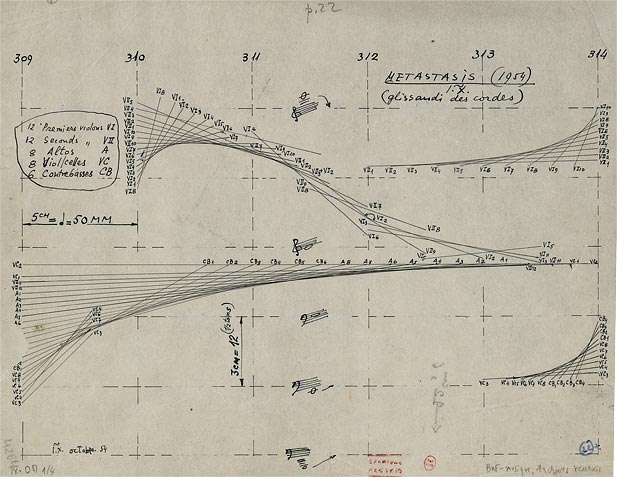
\includegraphics[width=\linewidth]{XenakisMetastasis.jpg}
  \caption{Excerpt from Iannis Xenakis' composition,
    \textit{Metastasis} (1954), measures 309-314. This score in this
    image was then transcribed to sheet music for the orchestral
    performance.}
  \label{fig:metastasis}
\end{figure*}

\subsection{The Philips Pavilion}
\label{sec:philips-pavilion-1}
\begin{figure}[h]
  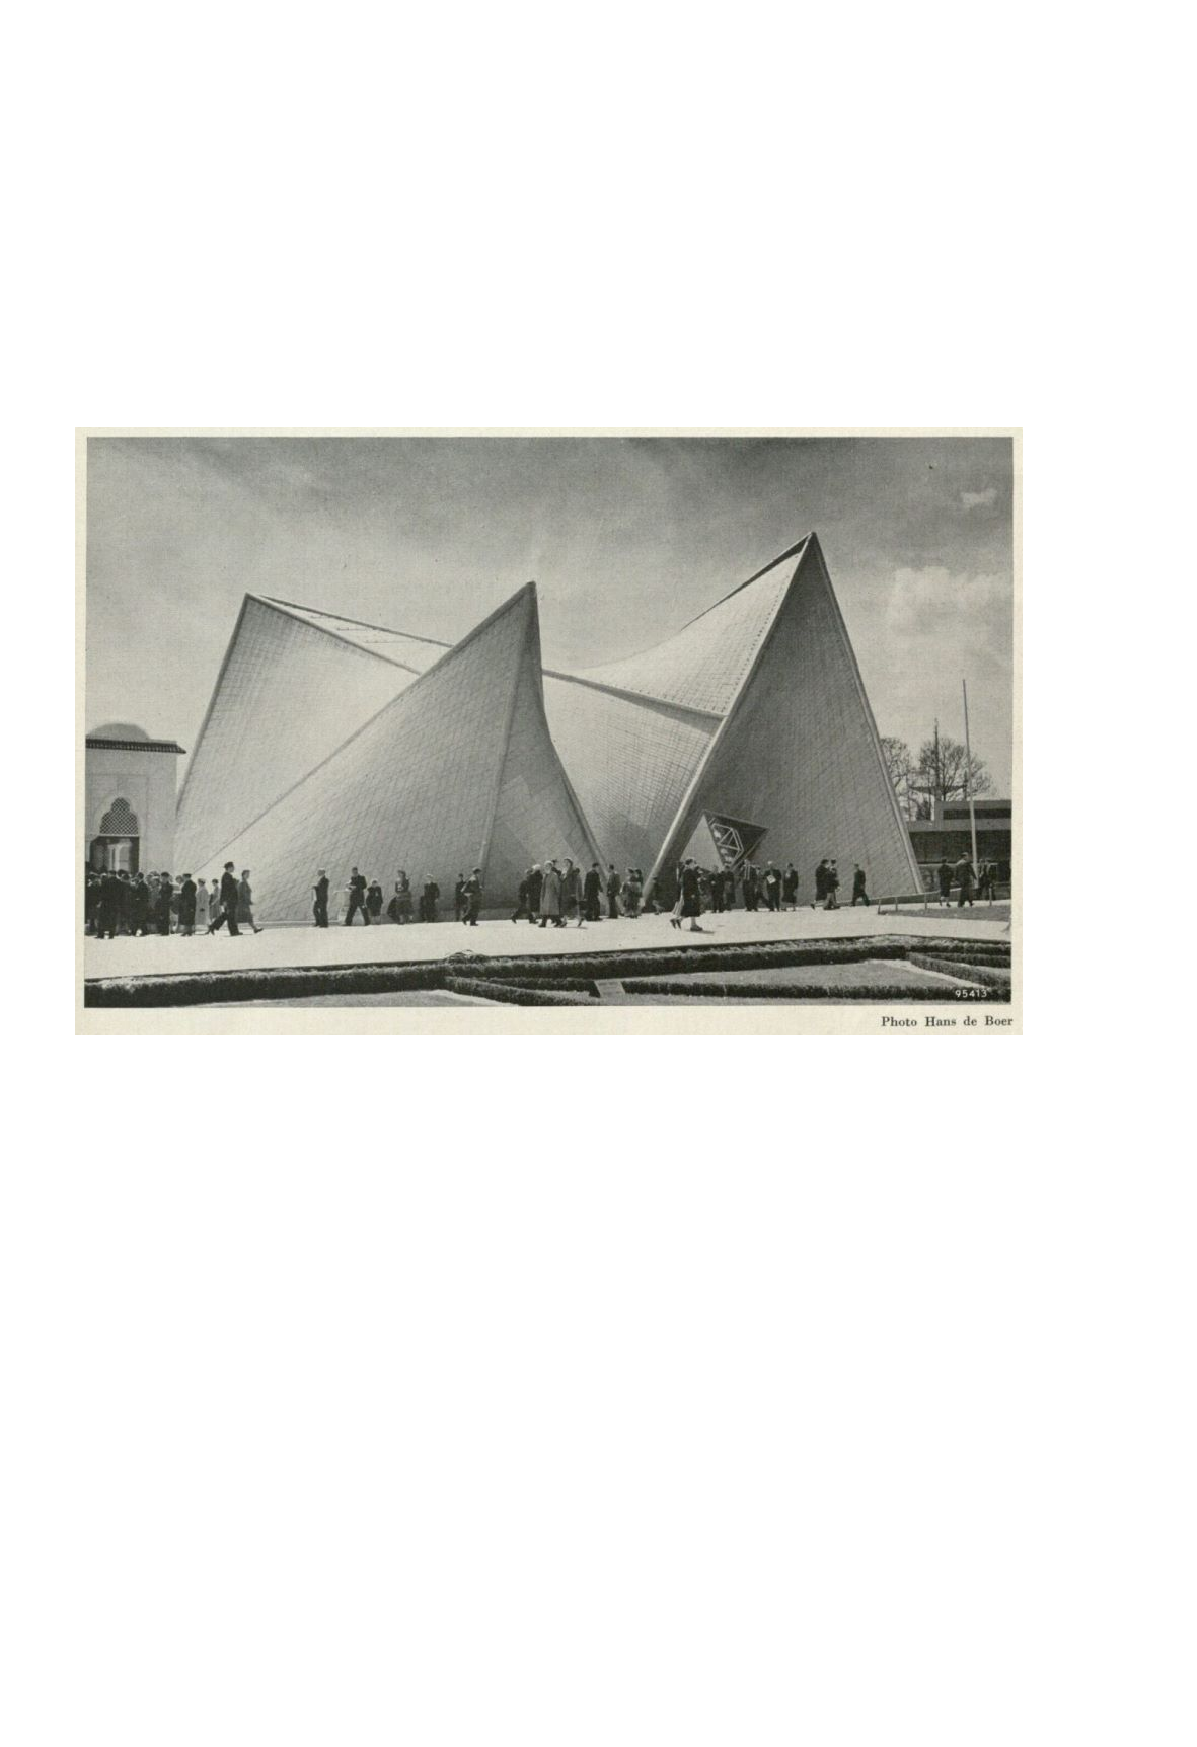
\includegraphics[width=\linewidth]{PhilipsPavilion-TechnicalReview-00.pdf}
  \caption{The Philips Pavilion at the 1958 Brussels World Fair as
    shown in Volume 20 of the \textit{Philips Technical Review}, 1959.}
  \label{fig:philips-pavilion-photo}
\end{figure}
In 1956, Le Corbusier was approached by Louis Kalff (Artistic Director
for the Philips corporation) and asked to build a pavilion for the
1958 World's Fair in Brussels. The pavilion was to showcase the sound
and lighting potential of Philips' technologies. Le Corbusier
immediately accepted, saying:
\begin{quotation}
  ``I will not make a pavilion for you but an Electronic Poem and a
  vessel containing the poem; light, color image, rhythm and sound
  joined together in an organic synthesis.''\cite{Lopez2011} 
\end{quotation}
The final product lived up to Le Corbusier's initial description. It
included:\cite{Lombardo2009}
\begin{enumerate}
\item A concrete pavilion, designed by architect and composer Iannis
  Xenakis
\item \textit{Interlude Sonoire} (later renamed \textit{Concret PH}), a
  tape music composition by Iannis Xenakis, approximately 2 minutes
  long, played between performances, while one audience left the
  pavilion and the next audience arrived
\item \textit{Po\`{e}me \'{E}lectronique}, a three channel, 8 minute
  tape music composition by composer Edgard Var\`{e}se
\item A system for spatialized audio across more than 350 loudspeakers
  distributed throughout the pavilion
\item An assortment of colored lighting effects, designed by Le Corbusier in
  collaboration with Philips' art director, Louis Kalff
\item Video consisting mostly of black and white still images,
  projected on two walls inside the pavilion
\item A system for synchronizing playback of audio and video,
  with light effects and audio spatialization throughout the
  experience
\end{enumerate} 

\paragraph{Role of Iannis Xenakis} During the initial design stage, Le
Corbusier decided that the shape of the pavilion should resemble a
stomach, with the audience entering through one entrance and exiting
out another. He completed initial sketches of the pavilion layout and
then delegated the remainder of the design to
Xenakis.\cite{Clarke2012}

The architectural evolution of the pavilion from Le Corbusier's early
designs (figure~\ref{fig:le-corbusier-sketch}) to Xenakis' iterations
(figure~\ref{fig:xenakis-draw}), illustrates the profound impact that
Xenakis had on the project. An article in the \textit{Philips
  Technical Review}\cite{philips1958} gives a wonderfully detailed
account of Xenakis' process in restructuring the design:\sidenote{\TODO{Clean this section.}}
\begin{enumerate}
\item Xenakis was aware that parallel walls and concave spherical
  walls would both negatively impact audio perceptibility due to repeated
  or localized acoustic reflections.
\item To accommodate musical purpose of the space he decided to
  explore surfaces with varying curvature...
\item 
  \begin{marginfigure}
    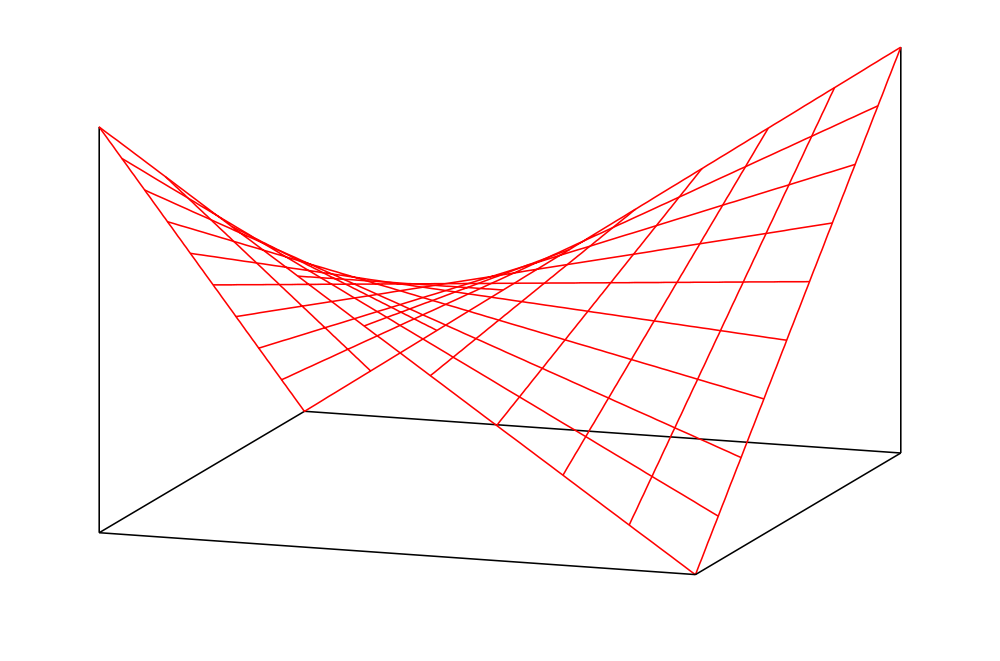
\includegraphics{hyperbolic-paraboloid}
    \caption{A ruled surface. For a surface to be considered ``ruled''
      every point on the surface must be on a straight line, and that
      line must lie on the surface. In Xenakis' time, ruled surfaces
      were useful in architecture, because they simplified the
      construction of curved surfaces by using straight beams.}
    \label{fig:ruled-surface}
  \end{marginfigure}...leading him to consider ruled surfaces such as
  the conoid and hyperbolic paraboloid. 
\end{enumerate}
Through this process, we see Xenakis utilizing the skills that he
learned at the Polytechnic Institute and continued to develop while
working with Le Corbusier. He also understood the mathematical
formation of the ruled surfaces that make up the structure. These
surfaces even look familiar to the Metastasis score
(figure~\ref{fig:metastasis}). In his 1963 book, \textit{Formalized
  Music}, Xenakis explicitly states that the Philips Pavilion was
inspired by his work on \textit{Metastasis}.

\begin{figure*}[]
  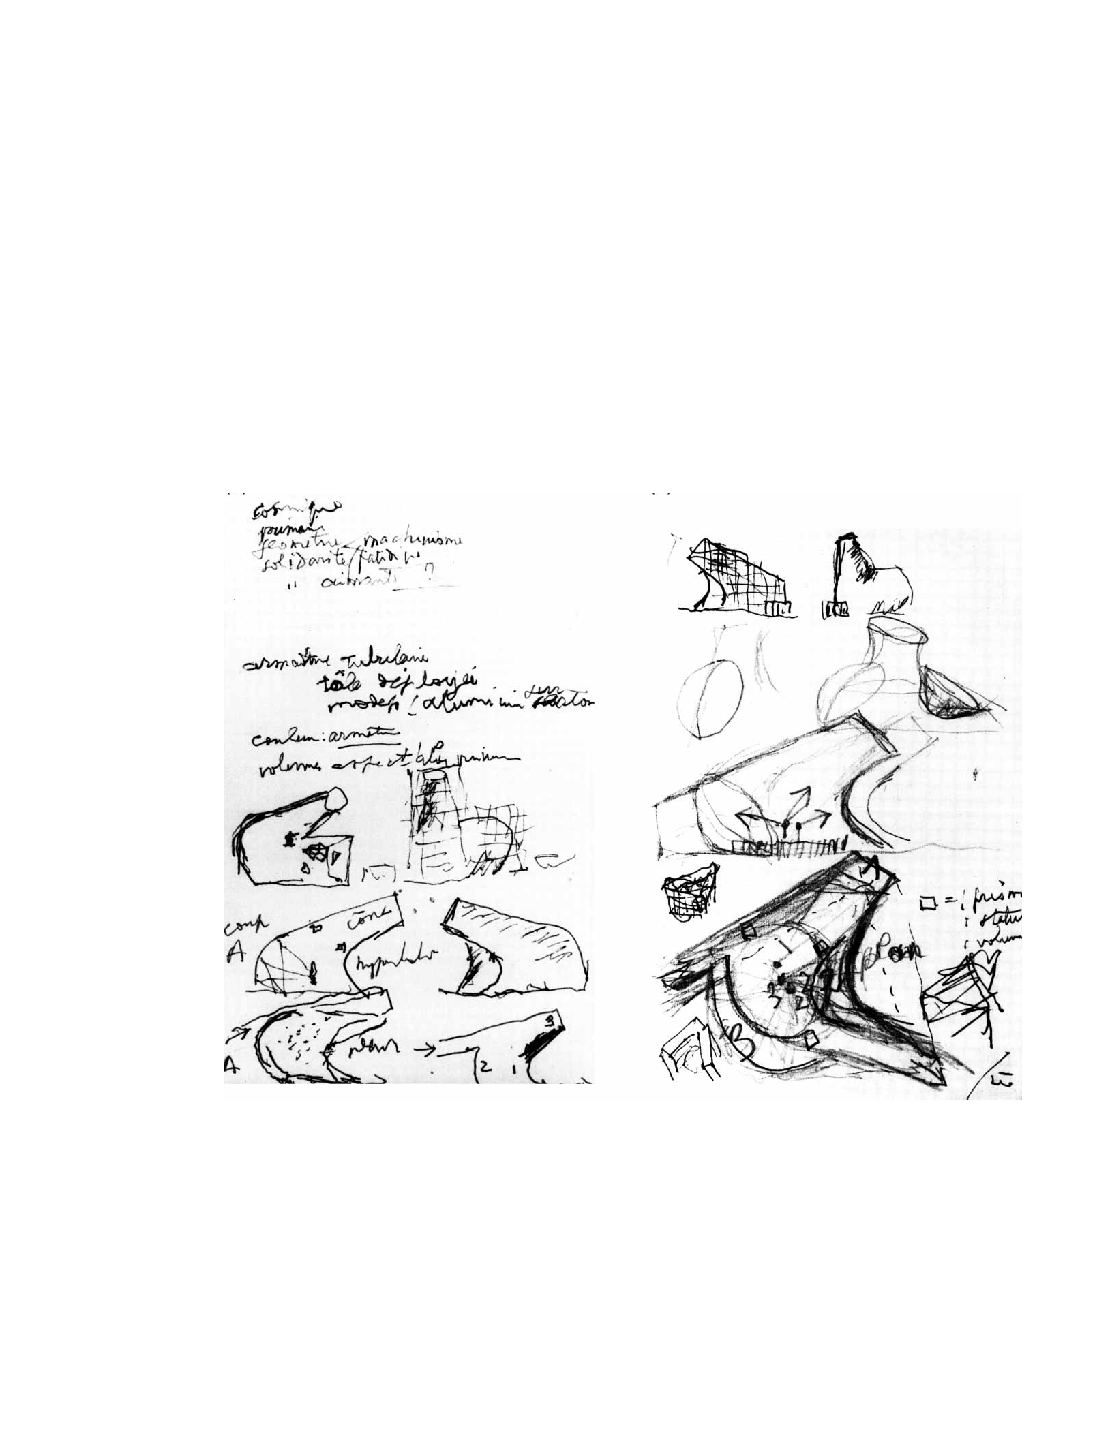
\includegraphics[width=\linewidth]{LeCorbusierDraw.pdf}
  \caption{Le Corbusier's design sketches for the Philips Pavilion,
    September \textendash{} October, 1956 (\textcircled{c} 2012
    Artists Rights Society, New York/ADAGP, Paris/FLC)}
  \label{fig:le-corbusier-sketch}
\end{figure*}

\begin{figure*}[h]
  % XenakisSketch.pdf or PhilipsDrawings.jpg
  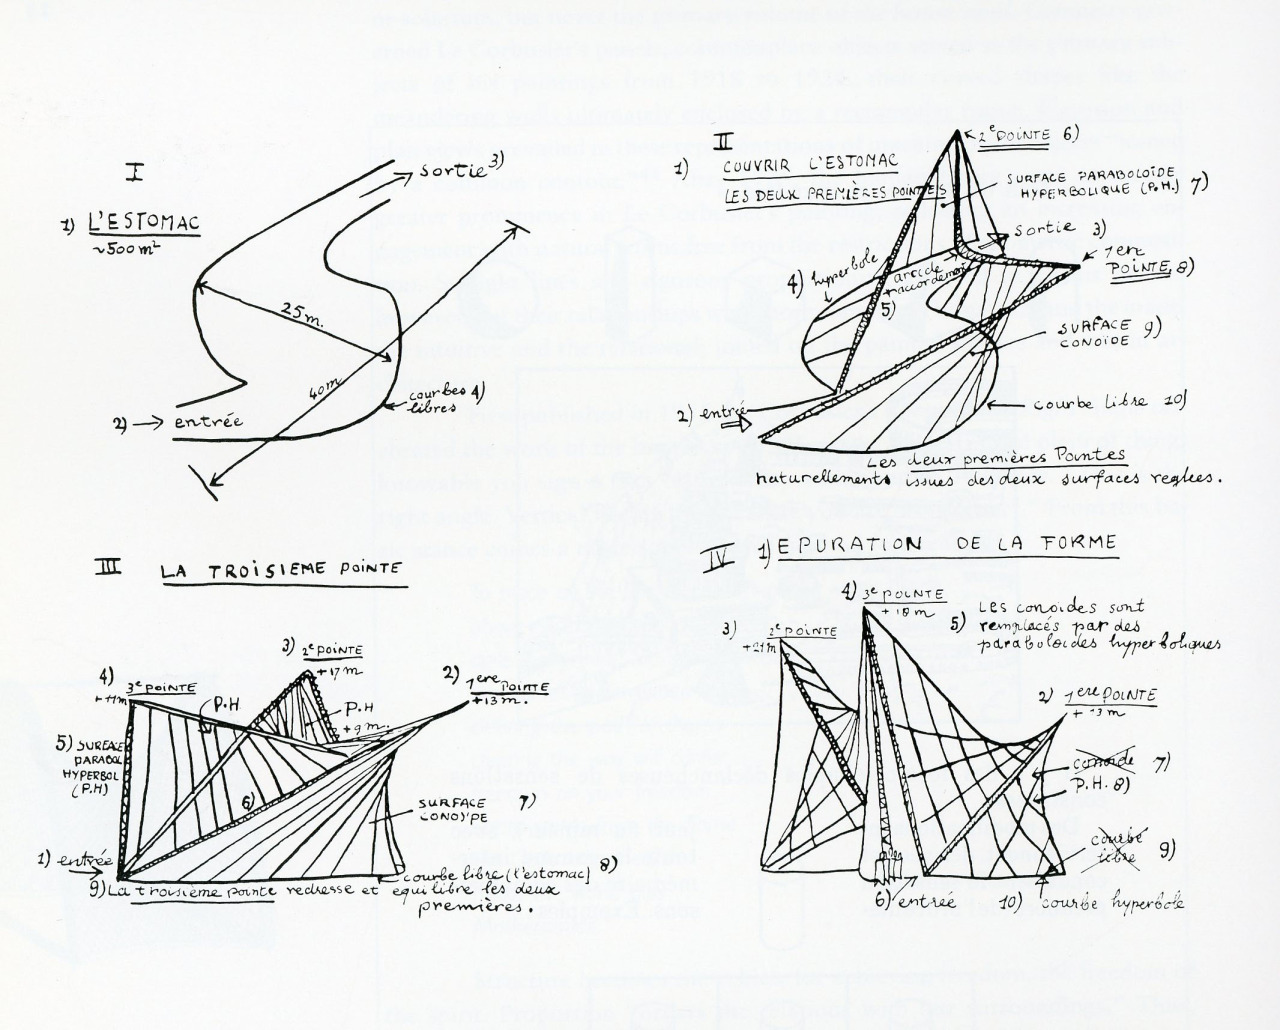
\includegraphics[]{PhilipsDrawings.jpg}
  \caption{Xenakis' early drawings of the Philips Pavilion as
    documented in volume 20 of the \textit{Philips Technical Review}.}
  \label{fig:xenakis-draw}
\end{figure*}

\section{Architecture and Music in Space and Time}
\label{sec:introduction-conclusion}

In \textit{Formalized Music}\cite{xenakis1992formalized}, Xenakis
describes how developments in music theory mimic equivalent
developments in philosophy, mathematics, and the sciences. Plato, for
example, believed that all events transpire as determined by cause and
effect. While Plato and Aristotle both described causality in their
writing, it was not until the 17th century that controlled experiments
and mathematics corroborated the theory.\sidenote{In 1687, Isaac
  Newton published \textit{Philosophi\ae{} Naturalis Principia
    Mathematica} (\textit{Mathematical Principles of Natural
    Philosophy}), in which he compiled the 3 laws of motion that set
  the foundation for the study of \emph{classical mechanics}.}
Similarly, music theory has historically employed causal rules to
describe counterpoint, tonality, and harmonic movement.\sidenote{\TODO{Add example}}

Causality was largely used to describe physical phenomena until the
19th century when statistical theories in physics began to include
probabilistic notions.\sidenote{The Maxwell-Boltzmann distribution,
  which was first derived by James Clerk Maxwell in 1860, describes
  the probability distribution for the speed of a particle within an
  idealized gas. For more see
  \url{http://plato.stanford.edu/entries/statphys-statmech/}} Xenakis
noticed that more contemporary fields like \emph{probability theory}
generalize and expand on the antecedent theories of causality. Xenakis
thought that music composition should naturally follow the progression
that physics did, with music theory generalizing and expanding on
causal rules that had existed previously. Indeed, starting in the late
19th century and early 20th century, composers like Strauss and
Debussy began to bend the existing rules of music theory, composing
music that branched away from the causal and tonal theories of the
time. With the rise of serialism\sidenote{Serialism is a technique for
  musical composition in which instances of musical elements (such as
  pitch, dynamics, or rhythm), are given numerical values. Sequences
  built from the values are ordered, repeated and manipulated
  throughout the composition.}  and indeterminate music\sidenote{In
  music, indeterminacy refers to the use of chance (such as rolling
  dice or flipping coins) as part of the compositional process.},
composers such as Stockhausen, Boulez, John Cage, Aaron Copland, and
B\'{e}la Bart\'{o}k began to use probability and chance in
composition, the same way that physicists were using probability to
describe the material world. 

To Xenakis' mind, serial music was no less causal than the music it
intended to supersede. He described serial music as embodying
``virtually absolute determinism.''\cite{xenakis1992formalized}
Xenakis saw music theory as a sub-set of mathematics and algebra:
While musicians have a different vocabulary, they also use
mathematical principles to describe and compose music. Because Xenakis
understood mathematics as well as music, he was able to identify how
even in serialism and indeterminate music, composers were only
utilizing a small subset of algebraic theory. In his own music,
Xenakis wanted to generalize and expand the causal framework that
musicians and theorists had been using to compose and understand
music, paralleling similar developments in physics and
mathematics. As a reference to \emph{chance}, or \emph{stochos},
Xenakis coined the term \emph{stochastic music} to describe his
development.\sidenote{\TODO{Clarify}}

Xenakis' book, \textit{Formalized Music} gives a verbose explanation
of stochastic music. Some authors have interpreted his description
more explicitly. In \textit{Audible Design}, Trevor Wishart describes
the stochastic process used to compose stochastic music as:
\begin{quotation}
  ``A process in which the probabilities of proceeding from one state,
  or set of states, to another, is defined. The temporal evolution of
  the process is therefore governed by a kind of weighted randomness,
  which can be chosen to give anything from an entirely determined
  outcome, to an entirely unpredictable one.''\cite{Wishart1994}
\end{quotation}
% It could be that the lack of a single clear definition by Xenakis is
% the reason that few composers today identify their work as stochastic
% music.

\paragraph{Xenakis' Reflection} In the Spring of 1976, while defending
his doctoral thesis at the University of Paris, Xenakis emphasized the
relevance of seemingly unrelated disciplines to the creative process. A
translation of his defense includes this statement:
\begin{quotation}
  ``The artist-conceptor will have to be knowledgeable and inventive
  in such varied domains as mathematics, logic, physics, chemistry,
  biology, genetics, paleontology (for the evolution of forms), the
  human sciences, and history; in short, a sort of
  \emph{universality}, but one based upon, guided by and oriented
  toward forms and architectures.''\cite{russolo1986art}
\end{quotation}
From Xenakis' drawings we can deduce that he used the same tools,
skills, and philosophy to imagine and conceive both music and
architecture. His approach elevated both forms and blurred the distinction
between the two. Perhaps if we had kept using pen and paper to design
buildings and write music, the reality today would be closer to the
ideal that he imagined. 

As the ideas that inspired Xenakis and other progressive 20th century
composers were taking root in contemporary music, the culture of
artistic form and composition was already beginning the transition
into the digital domain. There is no reason why digital tools cannot
favor stochastic processes to linearity; there is no reason why
digital tools cannot treat music and architecture as equals. However,
even today, software for composing music still favors static pitches
to glissandi; software for architectural design still favors corners
to curves. Most importantly, the software skills that we use to design
and manipulate space, and the skills that we use to compose music,
mutually exclude each other.

This is where the projects described here make a contribution.  By
drawing from music, mathematics, computer science, acoustics, audio
engineering and mixing, sound reinforcement, multimedia production,
and live performance, we can create tools that allow us to
indiscriminately compose with space and sound.

%%% Local Variables:
%%% mode: latex
%%% TeX-master: "CharlesHolbrow_MAS_Thesis"
%%% End:
